\chapter{非线性积分表达式化简}\label{ch06}
\section{问题的提出}
在非线性微分方程求解的过程中往往需要进行非线性积分表达式的化简. 因此, 本文将非线性积分化简作为一个具有挑战性的任务进行研究.

在 Maple 和 Mathematica 中, 只有当一个积分表达式的内部可以写成另一个表达式的导数时, 该积分才能被化简. 例如, 
\begin{equation}
\int\!{u_xv+uv_x \dd x}=\int\!{(uv)_x\dd x}=uv.
\label{complete_matched}
\end{equation}
我们称该类积分是\emph{完全匹配的}. 这类积分在其它的文献中也被称为是\emph{可积的}. 此外, Maple 只能化简单变量抽象函数的积分表达式, 而 Mathematica 能够化简多变量抽象函数的积分表达式. 

如果积分表达式的内部存在不匹配的项, 我们称它是\emph{非完全匹配的}. 例如,
\begin{equation}
\int\!{u_xv+2uv_x \dd x}=uv+\int\!{uv_x\dd x}.
\label{incomplete_matched}
\end{equation}
Maple 和 Mathematica 均不能化简上述积分表达式. 

利用 Maple 和 Mathematica 的内置函数可以化简\emph{完全匹配的}线性积分表达式. 但是, 对于积分的多项式, 问题将变得更加复杂. 如果一个多项式能够因式分解为多个线性表达式的乘积, 我们称它是\emph{线性可约的}. 对于这类积分多项式, 可以因式分解之后再用 Maple 和 Mathematica 的内置函数进行积分化简. 例如, 令$a=\int{u_x v \dd x},b=\int{u v_x \dd x},c=uv$, 可以得到一个\emph{线性可约的}表达式
\begin{equation}
a^2+2ab+b^2=(a+b)^2=c^2.
\label{liner_reducible}
\end{equation}

但是, 在一般情况下, 多项式并不是\emph{线性可约的}. 例如在同样的假设下, 我们有
\begin{equation}
a^2+3ab+b^2=(a+b)^2+ab=c^2+ab.
\label{non_linear_reducible}
\end{equation} 
我们称这种多项式是\emph{线性不可约的}. 目前没有任何算法能够解决这类积分化简问题. 因为这个问题的答案不是唯一的, 所以它比因式分解更加困难. 也就是说, 我们不能基于 Maple 和 Mathematica 的内置函数来化简这类问题. 

如果考虑嵌套积分, 问题将变得更加复杂. 例如, 
\begin{equation}
\int\!{\left(u\cdot\int\!{v_xw\dd x}+u\cdot\int\!{vw_x\dd x}\right)\dd x}=\int\!{uvw\dd x}.
\label{nested_integral}
\end{equation}
Maple 和 Mathematica 都不能化简这样的积分, 因为他们不能自动对积分内部进行因式分解. 有时, 一个嵌套积分需要被看作是一个导数才能完成化简. 例如,
\begin{equation}
\int\!{\left(u\cdot\int\!{v\dd x}+\int\!{u\dd x}\cdot v\right)\dd x}=\int\!{u\dd x}\cdot\int\!{v\dd x}.
\label{integral_as_differential}
\end{equation}
Maple 和 Mathematica 都不能化简这样的积分. 此外, \emph{非完全匹配}和\emph{线性不可约}的表达式可能递归地出现在积分的内部, 这使得化简问题变得越来越困难.

综上所述, 基于 Maple 和 Mathematica 的内置函数, 我们只能化简\emph{线性可约}且\emph{完全匹配}的积分表达式. 而本文将提出一个算法来化简更加一般的\emph{线性不可约}且\emph{非完全匹配}的积分表达式.

本章的组织结构如下: 在\refsec{Definitions-03}中, 我们将提出一些定义来更好的描述积分化简问题. 在\refsec{Simplify-03}中, 将描述我们算法的主要框架. 然后, 算法的关键细节将在\refsec{Details-03}中进行阐述. 接着, 本文将在\refsec{Results-03}中介绍 IntSimplify 软件包的实现, 同时分析它的时间复杂度和化简能力. 最终, 在\refsec{Conclusion-03}中对该算法进行小结.

\section{相关定义}\label{Definitions-03}
\begin{definition}
一个抽象函数的积分表达式(Abstract Integral Expression, 简称 AIE), 是由一些抽象函数(如$u(x,y),v(z,t)$), 在经过下列操作后得到的结果:
\begin{compactenum}[(1) ]
\item 关于自变量的积分;
\item 关于自变量的微分;
\item 上述结果的乘法;
\item 上述结果的线性组合;
\item 上述操作的迭代.
\end{compactenum}
\end{definition}

从而, 我们将AIE定义为一个代数结构. 而一个标准积分表达式(Standard Integral Expression, 简称SIE)则是将AIE展开至积分内部没有加法后的结果. 同时, 我们称SIE中的每一个加法项为标准积分项(Standard Integral Item, 简称SII). 它们的形式化定义如下:
\begin{definition}
设$\mathcal V$是自变量的集合, 而$\mathcal F$是定义在$\mathcal V$上的连续的抽象函数的集合. 对$\mathcal F$中的元素应用乘法\D 积分和微分操作之后, 得到的闭集记做$\mathbb F$. 对于任意的$f\in\mathbb{F}$, 我们称其为SII, 即
\begin{equation} 
f =\underbrace{\int\!\int\!\cdots\!\int}_m{ \frac{\partial^n}{\partial v_1 \partial v_2 \cdots \partial v_n} (g_1 g_2 \cdots g_l)\dd u_1 \dd u_2 \cdots \dd u_m}, 
\label{int_form}
\end{equation} 
其中 $u_1,\cdots,u_m,v_1,\cdots,v_n \in \mathcal V$, 而$g_1,\cdots,g_l \in \mathcal F$或和$f$具有相同的形式, 即$g_1,\cdots,g_l \in \mathbb F$.
\end{definition}

\begin{definition}
一个 SIE 是 SII 的线性组合, 即
\begin{equation}
I = \sum_{k=1}^N{c_k I_k}, 
\label{std_form}
\end{equation} 
其中 $c_k \in K$ and $I_k \in \mathbb F$. 
\end{definition}

SIE的定义不仅涵盖了一般的积分和微分表达式, 也涵盖了它们的乘法, 还涵盖了它们的嵌套积分. 由积分的线性性可知, 一个 AIE 一定能够通过展开加法得到 SIE.

基于抽象函数的连续性假设, 我们可以任意交换积分和微分的顺序. 类似地, 乘法也具有交换性. 为了在体现可交换性的同时简化SII的写法, 我们将\refeqn{int_form}重写为
\begin{equation} 
f=\partial^U_V(G),  \label{st_form}
\end{equation} 
其中 $U=[u_1,\cdots,u_m], V=[v_1,\cdots,v_n], G=[g_1,\cdots,g_l]$ 分别是积分变量\D 微分变量和积分项的无序列表. 当$U,V$为空或只含有一个元素时, \refeqn{st_form}在本文中有几个常用的简写形式:
\begin{equation}
\begin{split}
\partial_x&=\partial^\varnothing_{[x]},  \\
\partial^x&=\partial_\varnothing^{[x]},  \\ 
\partial(G)&=\partial^\varnothing_\varnothing(G).
\end{split}
\end{equation}
最后一个简写是为了区分积分项$\partial(G)$和无序列表$G$. 

从\refeqn{st_form}中可以看出, 一个SII被清晰的划分为三个组成部分. 为了从$f$中反向获取这三个部分, 我们定义了下列操作:
\begin{equation}
IV(f)=U,DV(f)=V,FC(f)=G.
\end{equation}
同时, 如果$f$只含有一个抽象函数, 我们记$TP(f)=simple$, 否则$TP(f)=complex$. 

将无序列表视为多重集, 就能基于集合的基本操作实现SII的乘法\D 积分和微分操作, 即:
\begin{equation}
\begin{split}
\partial(G_1)\cdot\partial(G_2)&=\partial(G_1+G_2),\\
\partial^{U'}_{V'}\partial^{U}_{V}(G)&=\partial^{U+U'}_{V+V'}(G).
\end{split}
\label{ops}
\end{equation}
这里, $+$是并集操作. 递归地应用上述操作可以压缩SII的结构, 使得$TP(f)=complex$蕴含$|FC(f)|\ge 2$. 

基于上述定义, 我们将一个积分多项式表示为SII的线性组合, 且关于SII的乘法\D 积分和微分操作能够用多重集的集合操作来实现. 

\section{算法核心框架} \label{Simplify-03}
我们的算法的目标在于将给定的AIE进行等价变换并使其最简. 首先, 本文将在\refsec{all_rules-03}中找到一系列的合并规则. 然后, 在\refsec{optimization-03}找到最优的化简的方案. 事实上, 该化简问题能够表示为一个$\ell_0$-优化问题. 因为它是NP-hard的, 我们将求解一个近似的$\ell_1$-优化问题. 


\subsection{寻找所有二项合并规则}\label{all_rules-03}
一般而言, 积分化简中的合并规则有无穷多种不同的形式, 如$u_x v + u v_x = (uv)_x$, $u_x v w+u v_x w + u v w_x = (uvw)_x$等等. 我们不可能一一列举所有情况. 但是, 从另一个角度来看, 所有多于二项的合并规则都能由二项的合并规则导出. 例如, $u_xvw+uv_xw+uvw_x=(uv)_xw+uvw_x=(uvw)_x$. 

对于最简单的二项合并规则$u_x v + u v_x = (uv)_x$, 可以对其进行乘法\D 积分和微分操作来构造新的合并规则. 忽略合并规则中的常数系数, 我们发现, 所有的二项合并规则都能写成$I_1+I_2=I_3$的形式, 其中 $I_1,I_2,I_3\in \mathbb F$. 因此, 可以基于最简单的二项合并规则获取所有可能的合并规则. 

设一个 SIE 中的所有SII构成集合$\mathcal I =\{I_1,\cdots,I_N\}$. 设集合$\mathbb I$满足$\mathcal I \subset \mathbb I$, 如果对于任意的$I_1,I_2\in \mathbb I$且$I_1+I_2=I_3$都有$I_3\in \mathbb I$, 我们称$\mathbb I$是$\mathcal I$的\emph{生成集}. 设$\mathbb I=\{B_1,\cdots,B_M\}$, 所有的合并规则就能构成集合$\mathcal R=\{{J_1}_l+{J_2}_l={J_3}_l|{J_1}_l,{J_2}_l,{J_3}_l \in \mathbb I, l=1..L\}$.

构造集合$\mathcal R$的算法如\refalg{FindAllRules}所示, 其中$FindRulesIn(I)$表示在$\{(I_1,I_2)|I_1, I_2 \in I\}$中寻找合并规则, 而$FindRulesBetween(I,J)$则表示在$\{(I_1,I_2)|I_1\in I, I_2 \in J\}$中寻找合并规则. 

\begin{algorithm}
\caption{IntSimplify: 寻找所有二项合并规则}
\label{FindAllRules}
\KwIn{一个SIE}
\KwOut{所有二项合并规则构成的集合}
\Fn{$FindAllRules(e)$}{
    $I\gets$ set of SIIs in $e$; $R\gets FindRulesIn(I)$\;
    \While{$\bf{true}$}{
        $J\gets$ new SIIs in $R$\;
        \lIf{$J=\emptyset$}{$\bf{break}$}
        $R\gets R \cup FindRulesIn(I) \cup FindRulesBetween(I,J)$\;
    }
    \Return{$R$}\;
}
\end{algorithm}

\refalg{FindAllRules}的时间复杂度直接决定了本文积分化简算法的复杂度. 该算法的复杂度取决于生成集$\mathbb I$中的元素个数. 记生成集的元素个数为$N$, 则该算法的复杂度是$\mathcal O(N^2)$. 尽管$N$的大小无法根据输入表达式直接确定, 但是可以估计它的最差情况. 考虑
\begin{equation}
I_n=\int\!{(f_1\cdot f_2\cdots f_n)_x \dd x},
\label{worst_case}
\end{equation}
其中$f_1,f_2,\cdots,f_n$是互不相同的抽象函数. \refeqn{worst_case}在展开后有$n$个积分项, 这些项构成了集合$\mathcal I$. 集合$\mathcal I$的任一非空子集中的项都能够合并, 合并后都能生成$\mathbb I$中一个不同的项. 因此, $N=2^n-1$. 所以\refalg{FindAllRules}的时间复杂度为$\mathcal O(4^n)$. 从而, 我们可以将 SII 中最大的相异函数个数定义为输出表达式的阶数. 于是, 该算法关于输入表达式的阶数的时间复杂度是指数的. 

\subsection{化简对应的优化问题}\label{optimization-03}
一旦建立了集合$\mathcal R$, 化简问题就能表示为一个等价变换
\begin{equation}
I=\sum_{k=1}^N{c_k I_k}-\sum_{l=1}^L{x_l ({J_1}_l+{J_2}_l-{J_3}_l)},
\label{normal_simplify}
\end{equation}
其中${J_1}_l+{J_2}_l={J_3}_l(l=1..L)$是集合$\mathcal R$中的元素. 然后, 化简问题就能转化为选择最优$x_l~(l=1..L)$的优化问题.

一般情况下, 化简是为了最小化项数或最简化系数. 为了更好的表达这两个目标, 我们可以将\refeqn{normal_simplify}转化为矩阵形式. 

设 
\begin{equation}
\begin{split}
\sum_{k=1}^N{c_k I_k} &= \sum_{k=1}^M{b_k B_k},\\
\sum_{l=1}^L{x_l ({J_1}_l+{J_2}_l-{J_3}_l)} &= \sum_{j=1}^L{x_j \sum_{i=1}^M{a_{ij} B_i}}.
\end{split}
\end{equation} 
令$\bm B=(B_1,\cdots,B_M),\bm b=(b_1,\cdots,b_M)\TT,\bm x=(x_1,\cdots,x_L)\TT,\bm A=(a_{ij})_{M \times L}$, \refeqn{normal_simplify}可以写成 
\begin{equation}
I=\bm{B}\bm{b}-\bm{B}\bm{A}\bm{x}=\bm{B}(\bm{b}-\bm{A}\bm{x}).
\end{equation}

为了最小化项数, 我们需要做一个$\ell_0$-优化
\begin{equation}
    \underset{\bm x}\min~\VecNorm{\bm{b}-\bm{A}\bm{x}}_0,
\end{equation}
其中$\VecNorm{\bm x}_0$是$\ell_0$-范数. 因为这个问题是NP-hard的, 我们可以求解另一个相对简单的近似优化问题
\begin{equation}
\underset{\bm x}\min\VecNorm{\bm{b}-\bm{A}\bm{x}}_1.
\label{LAE}
\end{equation}
在这个问题中, 我们不仅能够近似地最小化项数, 还能最简化系数. 

事实上, $\ell_1$-优化能够转化为一个线性规划\cite{L1_regression}, 即
\begin{equation}
\begin{split}
&\underset{\bm u,\bm x}\min \sum_{k=1}^L{u_k},\\
&s.t. \left\{
\begin{matrix}
\bm{u}\ge \bm{b}-\bm{A}\bm{x},\\ 
\bm{u}\ge \bm{A}\bm{x}-\bm{b},
\end{matrix}
\right.
\end{split}
\label{LP}
\end{equation}
其中 $\bm u=(u_1,\cdots,u_L)\TT$. 这些约束条件能够使得问题在求得最优解时满足$\bm u = |\bm{b}-\bm{A}\bm{x}|$. 于是, 该优化问题和原问题是等价的. 同时, 该问题又不包含绝对值操作, 所以它能够被线性规划算法求解. 

最终, 我们将积分化简的问题转换为一个线性规划问题进行求解.

\section{关键的子算法} \label{Details-03}
\subsection{寻找二项合并规则的子算法} \label{Combine-03}
如前文所述, 所有的合并规则都是由两个SII的合并规则构造而成的. 在本节中, 我们将介绍寻找两个SII间合并规则的关键算法. 

对于最简单的合并规则$u_x v + u v_x = (uv)_x$, 可以在其上做乘法\D 积分和微分操作来构造新的合并规则. 反之, 任意的合并规则都能归结为最简单的情况. 

设$I_1,I_2$是两个SII, 考虑 
\begin{equation}
\begin{split}
I_1+I_2 &= \partial^U_V(j_1) + \partial^U_V(j_2) \\
        &= \partial^U_V( j_1+j_2 )\\
        &= \partial^U_V( f\cdot(j_3+j_4) )\\ 
        &= \partial^U_V( f\cdot r ) = I_3 .
\end{split}
\label{combine_form}
\end{equation} 
第二个等式在$I_1,I_2$具有相同积分和微分变量时成立, 即$IV(I_1)=IV(I_2),DV(I_1)=DV(I_2)$. 而积分项的内部$j_1,j_2$的公共部分在第三个等式中被提取为$f$, 剩余部分分别为$j_3$和$j_4$. 若$j_3,j_4$能够合并则将得到最终的合并结果. 

如果第三个等式在积分外部成立, 则代表了这样的情况: 
\begin{equation}
f\cdot\int\!{u_x v\dd x}+f\cdot\int\!{u v_x \dd x} = f\cdot(uv).
\end{equation} 
因为$f$是任意的, 如果取$f=1$就对应了最简的线性合并规则. 如果$f$是多个积分项的乘积, 则涵盖了多项式的因式分解. 这表明我们的算法适用于积分多项式. 

如果第三个等式在积分内部成立, 则代表了这样的情况:
\begin{equation}
\int\!{f \left(\int\!{u_x v\dd x}\right)\dd y}+\int\!{f \left(\int\!{u v_x \dd x}\right) \dd y} = \int\!{fuv\dd y}.
\end{equation}
这表明我们的算法也适用于含嵌套积分的情况. 

\refeqn{combine_form}中的$j_3+j_4=r$需要分两种情况进行考虑: \emph{根情况}和\emph{递归情况}. 

\emph{根情况}表示$j_3+j_4$能够通过最简单的二项合并规则进行合并, 即
\begin{equation}
\begin{array}{rl}
& j_3+j_4=u \cdot v+\partial^x(u)\cdot \partial_x(v) = \partial^x(u)\cdot v, \\
\text{或}& j_3+j_4=u \cdot v+\partial_x(u)\cdot \partial^x(v) = \partial^x(v)\cdot u.
\end{array}
\label{root_form}
\end{equation}

\emph{递归情况}则表示$j_3+j_4$是通过递归地使用\refeqn{combine_form}完成合并的. 该情况意味着$j_3$和$j_4$都是积分项, 而不是积分项的乘积.

这两种情况都要求\red{每个积分项的内部至少有两个乘法项}. 因此, 我们有$TP(I_1)=TP(I_2)=complex$.  

基于上述分析, 我们给出了\refalg{FindRuleForPair}. 对于输入的$I_1,I_2$, 我们首先验证其是否满足\emph{根情况}和\emph{递归情况}的公共条件. 然后, 设$I_1,I_2$的内部分别为$J_1,J_2$, 基于集合操作提取它们的公共部分$F$和剩余部分$J_3,J_4$. 最终, 我们先尝试对$J_3,J_4$进行直接合并. 若合并失败且$|J_3|=|J_4|=1$, 则尝试对它们进行递归合并.  

\begin{algorithm}
\caption{IntSimplify: 寻找两个SII的合并规则}
\label{FindRuleForPair}
\KwIn{标准积分项$I_1,I_2$, 外部积分变量的集合$S$.}
\KwOut{如果$I_1 + I_2 = I_3$则返回$I_3$, 否则返回$FAIL$.}
\Fn{$FindRuleForPair(I_1,I_2,S)$}{
    \tcp{检查公共条件}
    \lIf{\bf{not} $( TP(I_1)=TP(I_2)=complex$  \bf{and} $IV(I_1)=IV(I_2)$ \bf{and} $DV(I_1)=DV(I_2) )$}{
        \Return{$FAIL$}
    }
    \tcp{初始化}
    $U \gets IV(I_1), V\gets DV(I_1),S\gets U \cup S $\;
    $J_1\gets FC(I_1), J_2\gets FC(I_2) $ \;
    $F\gets J_1 \cap J_2, J_3\gets J_1-F, J_4\gets J_2-F$\;
    \tcp{保证$|J_3|\le |J_4|$}
    \lIf{$|J_3|>|J_4|$}{
        $J_3,J_4\gets J_4,J_3$
    }
    \tcp{尝试直接合并}
    \uIf{$\min(|J_3|,|J_4|)=1$}{
        $r,F\gets FindRuleForVars1(\partial(J_3),\partial(J_4),F,S)$\;
    }\uElseIf{$\min(|J_3|,|J_4|)=2$}{
        $r\gets FindRuleForVars2(\partial(J_3),\partial(J_4),S)$\;
    }\lElse{
        $r\gets FAIL$
    }
    \tcp{尝试递归合并}
    \If{$r=FAIL$ \bf{and} $|J_3|=|J_4|=1$}{
        $r\gets FindRuleForPair(\partial(J_3),\partial(J_4),S) $\;
    }
    \tcp{构造合并规则}
    \lIf{$r\neq FAIL$}{
        \Return{$\partial^U_V(\partial(F)\cdot r)$}
    }
    \Return{$FAIL$}\;
}
\end{algorithm}

上述数学化描述和伪代码中算法化的描述主要存在以下三处差异:

(一) 我们在代码中使用多重集来代替SII进行计算. \red{伪代码中多重集的变量名是数学描述中对应名称的大写}.

(二) 其实, \emph{根情况}需要细分为两种情况进行讨论:
\begin{asparaenum}[(i)]
\item \emph{一般根情况}: 一般情况下, $|J_3|=|J_4|=2$, 我们可以根据\refeqn{root_form}来寻找合并结果. 如果 
\begin{equation}
j_1+j_2 = f \cdot ( u \cdot (v_1 \cdots v_n)_x +  u_x \cdot (v_1 \cdots v_n ) ), 
\end{equation}
则有 $|J_3|=2,|J_4|=n+1\ge 2$. 这样的情况也能被和$|J_3|=|J_4|=2$一样的程序所处理, 所以我们将这两种情况归结为$\min(|J_3|,|J_4|)=2$. 这两种情况能够被\refalg{FindRuleForVars2}所处理.
\item \emph{特殊根情况}: 在特殊情况下, 可能有
\begin{equation}
\begin{split}
j_1 + j_2   &= f \cdot ( j_3 g + j_4 g ) \\ 
            &= f \cdot ( (g \cdot t_1\cdots t_n)_x\cdot g + (g \cdot t_1\cdots t_n)\cdot g_x ),
\end{split}
\end{equation}
其中$j_3=(g \cdot t_1\cdots t_n)_x , j_4=t_1\cdots t_n\cdot g_x$. 我们有$\min(|J_3|,|J_4|)=1$. 在这种情况下, $TP(j_3)=complex, g\in FC(j_3)\cap F$. 所以, 在\refalg{FindRuleForVars1}中我们对所有可能的$g$都进行了尝试. 
\end{asparaenum}

\begin{algorithm}
\caption{IntSimplify: 一般根情况合并} 
\label{FindRuleForVars2}
\Fn{$FindRuleForVars2(I_1,I_2,S)$}{
    $[u,v]\gets FC(I_1)$\tcp*[l]{Extract contents of multiset.}
    \For{$x\in S\cap FV(I_1) \cap FV(I_2)$}{
        \lIf{$\partial_x(u) \cdot \partial^x(v)=I_2$}{
            \Return{$\partial_x(u \cdot \partial^x(v) )$}
        }
        \lElseIf{$\partial^x(u) \cdot \partial_x(v)=I_2$}{
            \Return{$\partial_x(\partial^x(u) \cdot v )$}
        }
    }
    \Return{$FAIL$}\;
}
\end{algorithm}

\begin{algorithm}
\caption{IntSimplify: 特殊根情况合并}
\label{FindRuleForVars1}
\Fn{$FindRuleForVars1(u,t,F,S)$}{
    \lIf{$TP(u)\neq complex$}{
        \Return{$FAIL,F$}
    }
    $G \gets FC(u) \cap F$\;
    \For{$v \in G$}{
        $I_1\gets u \cdot v,I_2 \gets t\cdot v$\;
        \For{$x \in S\cap FV(I_1) \cap FV(I_2)$}{
            \uIf{$\partial_x(u) \cdot \partial^x(v)=I_2$}{
                $F\gets F-[v]$\;
                \Return{$\partial_x(u \cdot \partial^x(v) ),F$}\;
            }
            \ElseIf{$\partial^x(u) \cdot \partial_x(v)=I_2$}{
                $F\gets F-[v]$\;
                \Return{$\partial_x(\partial^x(u) \cdot v ),F$}\;
            }
        }
    }
    \Return{$FAIL,F$}\;
}
\end{algorithm}

(三) 在算法中存在一个额外参数$S$. 这个参数表示当前递归下, 外部所有积分变量的并集. 我们知道, 如果没有外部的积分, 像$u_x v + u v_x = (uv)_x$这样的表达式在合并之后也会被自动展开. 默认情况下, 对于像$\int\!{u_x v\dd x} + \int\!{u v_x\dd x} = uv$一样的积分, 我们取$S=\varnothing$. 但是, 如果想合并没有外部积分的微分表达式, 我们可以取$S$为所有自变量的集合$\mathcal{V}$.  

在\refalg{FindRuleForVars2}和\refalg{FindRuleForVars1}中, 我们仅在$S$上寻找合并规则. 又因为$u_x v + u v_x = (uv)_x$要求$x$是$u$和$v$的自变量. 所以我们只需要在$S\cap FV(I_1) \cap FV(I_2)$上寻找合并规则即可. 这里, $FV(f)$是$f$内部的公共因子, 满足
\begin{equation}    
FV(f)=\left\{
\begin{array}{cl}
\bigcap\limits_{g\in FC(f)}{FV(g)}, &\text{if }TP(f)=complex;\\ 
f\text{的自变量集合},          &\text{if }TP(f)=simple.
\end{array}
\right.
\end{equation}

综上所述, 我们已经描述了寻找二项合并规则的所有细节. 现在我们给出一个典型的例子来演示我们的算法是如何工作的.

\begin{example} \label{eg-4-1}
令
\begin{equation}
a=\int\!{uu_xv \dd x},~~b=\int\!{u^2v_x\dd x},~~c=\int\!{u(uv)_x\dd x},~~d=u^2v.
\end{equation}
其所有的二项合并规则为$\{a+b=c,a+c=d\}$. 

对于$a+b=c$, 我们有$F=[u],J_3=[u_x,v],J_4=[u,v_x]$, 它能够被\refalg{FindRuleForVars2}合并.

对于$a+c=d$, 我们有$F=[u],J_3=[(uv)_x],J_4=[u_x,v]$, 它能被\refalg{FindRuleForVars1}合并.  

对于\emph{不完全匹配}的表达式$3a+b$, 通过求解对应的优化问题, 我们可以得到其最简结果为$a+d$.

对于\emph{线性不可约}的多项式$5a^2+4ab+b^2$, 我们可以找到如下8条二项合并规则: 
\begin{equation}
\begin{matrix}
a^2+ab=ac, &ab+b^2=bc, &ac+bc=c^2, &ac+c^2=cd,\\
ad+bd=cd,  &a^2+ac=ad, &ab+bc=bd,  &ad+cd=d^2.
\end{matrix}
\end{equation}
这些合并规则共有10个不同的SII, 且他们都能够通过\refalg{FindRuleForPair}的\emph{递归情况}获得. 

对于这些规则, 以$a^2+ab=ac$为例, 我们在第一层递归时有$F=[a],J_3=[a],J_4=[b]$, 这属于因式分解. 在第二层递归中, 基于\emph{根情况}可以得到$a+b=c$. 最终, 通过求解对应的优化问题, 我们可以得到$5a^2+4ab+b^2$的最简结果为 $a^2+d^2$.
\end{example}  

\subsection{优化算法的有关细节}\label{optMethods-03}

如\refsec{optimization-03}所述, 积分化简的问题能够转化为一个线性规划(Linear Programming, 简称LP)问题进行求解. 但是, 我们的问题不能直接用数值的LP算法求解. 因为, 一旦存在数值误差, 就会产生很多系数很小的冗余项, 且很难判断这些项是真实存在的还是由数值误差造成的. 所以, 我们要用精确线性规划(Exact Linear Programming, 简称ELP)算法进行求解. 

现有的ELP算法有: Maple中的\cd{simplex}\D Mathematica 中的\cd{LinearProgramming}\D \spell{SoPlex}\cite{soplex}和\spell{Qsopt-ex}\cite{qsoptex}等. 并且, 这些 ELP 算法都是针对有理数域上的问题进行求解的, 因此需要将我们的问题转化到有理数域上. 

回顾\refeqn{std_form}中SIE的定义, 我们假设系数$c_k\in K$, 且标准积分项$I_k\in \mathbb F$. 我们的化简问题所属的范围由这两个集合所确定, 因此, 用$K[\mathbb F]$来表示我们的问题. 一般情况下, 我们需要求解$\mathbb C[\mathbb F]$, 即允许系数是复数. 将虚数单位$i$看作一个常数, 我们有$\mathbb C[\mathbb F]=\mathbb R[\mathbb F \cup \{i\}]$. 此外, 将所有无理数也视为常数, 我们有$\mathbb C[\mathbb F]=\mathbb Q[F\cup (\mathbb R - \mathbb Q) \cup \{i\}]$. 最终, 我们将问题转化到了有理数域上. 

\begin{example}
考虑
\begin{equation}
\left(1+\sqrt{2}\right)\ii{u_x v}+\sqrt{2}\ii{u v_x}, 
\end{equation}
我们有 
\begin{equation}
\bm{B}=\left(
\begin{array}{c}
\ii{u_x v}  \\
\ii{u v_x}  \\
u v         \\
\sqrt{2}\ii{u_x v}  \\
\sqrt{2}\ii{u v_x}  \\
\sqrt{2}u v         \\
\end{array}
\right)\TT,
\bm{b}=\left(
\begin{array}{c}
1   \\
0   \\
0   \\
1   \\
1   \\
0   \\
\end{array}
\right),
\bm{A}=\left(
\begin{array}{rr}
1   & 0\\
1   & 0\\
-1  & 0\\
0   & 1\\
0   & 1\\
0   & -1\\
\end{array}
\right).
\end{equation}
求解对应的ELP, 其最优解为$\bm{x}=\left(0,1\right)\TT$. 于是, 最优的化简结果为$\sqrt{2}uv+\ii{u_x v}$. 
\end{example}

事实上, 对于有理数域上的化简问题, 在提取公共分母之后, 就能使得系数都为整数, 此时化简问题显然有整数解. 因此, 另一个避免数值误差的方法是用数值整数线性规划(Numerical Integer Linear Programming, 简称NILP)替代ELP. 只需对求解结果取整就能简单的避免数值误差. 在理论上 ILP 是要难于LP的, 因为 ILP 是NP-hard的. 但是, 由于数值算法在运行时比符号算法更快, NILP 也有可能比 ELP 快. 

基于上述考虑, 我们在程序中集成了下列优化算法: 
\begin{compactitem}[\textbullet]
\item \cd{SLP}: 表示 Maple 中的\cd{simplex}, 是一个ELP算法; 
\item \cd{mmaSLP}: 表示 Mathematica 中的\cd{LinearProgramming}, 是一个ELP算法;
\item \cd{SoPlex}\cite{soplex}: 是一个用C++实现的ELP算法;
\item \cd{NILP}: 表示 Maple 中的\cd{LPSolve}, 是一个NILP算法;
\item \cd{MatlabILP}: 表示 Matlab 中的 \cd{intlinprog} , 是一个 NILP 算法.
\end{compactitem}

现在, 我们用一个具体的例子来比较这些算法在不同规模的问题下的运行时间. 令$\mathcal F=\{f_1,f_2,\cdots\}$, 考虑
\begin{equation}
\left(\sum\limits_{k=1}^{n_1}{\int\!{(f_{i_{2k-1}}f_{i_{2k}})_x\dd x}}\right)^2+\sum\limits_{k=1}^{n_2}{\int\!{(f_{j_{3k-2}}f_{j_{3k-1}}f_{j_{3k}})_x\dd x}},
\end{equation}
其中 $i_k,j_k \in \{1,2,\cdots\}$. 为了控制生成的积分项的数量, 我们在实验中取$n_1\le 8,n_2\le 8$. 求解优化问题的时间如\reffig{opts_log}所示. 为了更清晰地进行比较, 我们在作图时对运行时间取了对数. 

\begin{figure}[htbp]
\centering
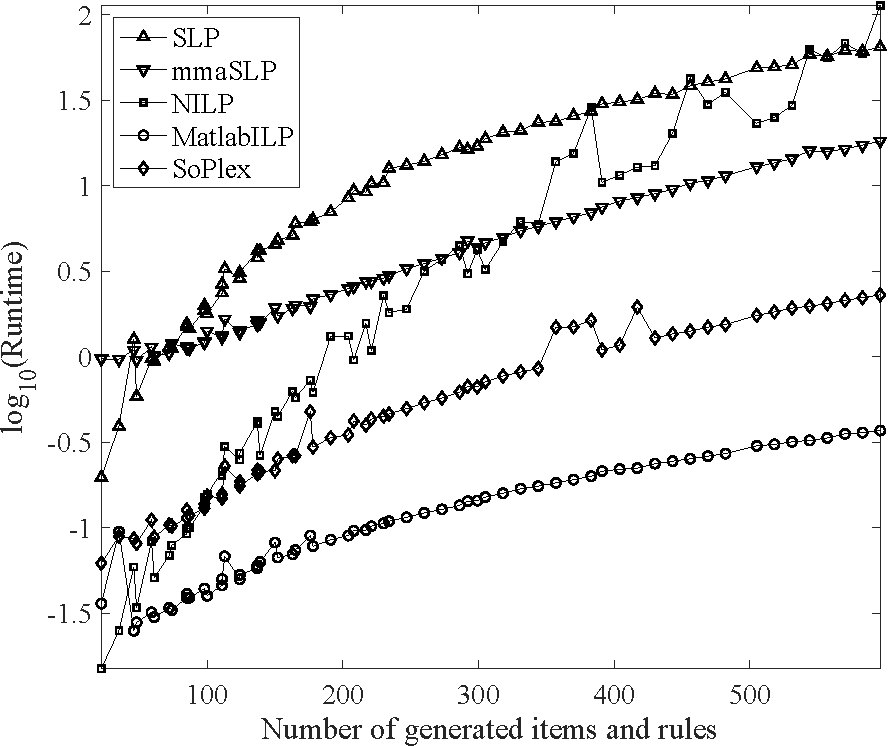
\includegraphics[width=0.75\textwidth]{fig/int-6.pdf}
\caption{优化算法的运行时间}\label{opts_log}
\label{opts_all}
\end{figure}

在\reffig{opts_all}中可以看出, ELP算法运行时间的增长趋势是相似的. 但是, \cd{SoPlex}比其它ELP算法都快. 在我们的实验中, \cd{SoPlex}的运行时间始终在2秒以内. 

尽管 ILP 要比 LP 更难, 但是数值计算的优势使得 NILP 算法比 ELP 算法更快. 例如, 在问题规模小于250时, \cd{NILP} 要比 \cd{SLP} 和 \cd{mmaSLP}更快. 而\cd{MatlabILP}则始终显著地快于\cd{SLP} 和 \cd{mmaSLP}. 从图中也可以看出, \red{Maltab 中 ILP 算法的效率要高于 Maple}. 这是因为 Matlab 在分支定界法\cite{wolsey1998integer}的基础上, 还集成了许多 LP 和 ILP 中的预处理技术\cite{preLP1995,preLP2003,preMILP1994,cut2008}, 同时还引入了许多优秀的启发式求解策略\cite{Heuristics2005,berthold2006primal}. 事实上, 除了 Matlab 以外, Gurobi 也是一个非常优秀的 ILP 求解器, 且它在一些复杂问题上性能要优于 Matlab. 但是, Gurobi 在本文的问题上性能优势不大, 为了简化本文软件包的依赖环境, 我们没有集成 Gurobi. 

此外, 很难说 \cd{MatlabILP} 比 \cd{SoPlex} 更快. 因为我们在调用 \cd{SoPlex}时使用的是命令行的接口, 这将在文件IO和程序启动上花费更多的时间.

总的来说, 在我们的问题中, \cd{SoPlex} 和 \cd{MatlabILP} 是最快的算法. 

\section{IntSimplify 软件包的实现与测试}\label{Results-03}
基于上文描述的算法, 我们实现了能够进行非线性积分表达式化简的软件包 IntSimplify. IntSimplify 有两个主要接口: \cd{IntExpand} 和 \cd{IntCombine}. \cd{IntExpand} 用于将输入的积分表达式转化为SIE, 而\cd{IntCombine} 则会进行积分的化简.

\cd{IntCombine}的调用方式为
\begin{verbatim}
IntCombine(e,{optMethod,CombineDiff});
\end{verbatim}
其中 
\begin{compactitem}[\textbullet]
\item \cd{e}表示输入的积分表达式.
\item \cd{optMethod}表示执行精确线性规划的算法, 它有以下几个可选的取值: \cd{SLP, mmaSLP, SoPlex, NILP}和\cd{MatlabILP}. 这些选项的意义和上文保持一致. 为了最小化程序运行的依赖环境, 同时考虑到求解的效率, \cd{optMethod}的默认值是\cd{NILP}. 
\item \cd{CombineDiff}是一个可选参数, 指定\cd{CombineDiff=true}能够让程序合并外部不含积分的微分表达式, 如$uv_x+u_xv=(uv)_x$. 默认情况下, \cd{CombineDiff=false}, 即程序只会合并类似于$\ii{u_xv}+\ii{uv_x}=uv$的表达式. 
\end{compactitem}

\cd{IntCombine}的实现逻辑如下:
\begin{compactenum}[Step 1.]
\item 首先, 调用\cd{IntExpand}将输入表达式转化为SIE.
\item 然后, 将 SIE 中的每个 SII 转化为\cd{IntFunc}对象. \cd{IntFunc}对象是基于前文定义所实现的, 它基于多重集的集合操作实现了SII的积分\D 微分和乘法操作. 值得说明的是, 我们还在 Maple 中自行实现了多重集数据结构. 虽然在Maple 2016以后的版本中, 存在名为\cd{MultiSet}的内置对象, \red{但是为了兼容Maple 18之后的版本}, 我们还是选择自行实现多重集数据结构.
\item 基于\refalg{FindAllRules}\D \refalg{FindRuleForPair}\D \refalg{FindRuleForVars1} 和\refalg{FindRuleForVars2}, \red{找到所有的二项合并规则}.
\item 基于找到的二项合并规则, 将化简问题转化为精确线性规划问题进行求解. 在求解时调用用户指定的算法进行优化. 各个算法的调用方式如下:
\begin{compactitem}[\textbullet]
\item \cd{SLP}和\cd{NILP}直接调用 Maple 内置函数.
\item \cd{mmaSLP}将对应的问题转化为 Mathematica 命令之后, 通过命令行接口调用.
\item \cd{SoPlex}将C++源码编译为可执行文件之后, 将对应的问题输出到特定格式的文件, 再调用命令行接口进行求解.
\item \cd{MatlabILP}是通过Maple的\cd{Matlab}软件包调用的. 在启动 Matlab 服务之后, Maple 将 Maltab 命令发送到 Maltab 服务进行求解. 该调用过程在第一次启动 Matlab 时比较耗时, 之后的调用时间则可以忽略不计.
\end{compactitem}
\item 最后, 我们将优化结果还原为积分表达式并输出.
\end{compactenum}

基于 IntSimplify, 我们将在\refsec{sec5.1-03}中分析本文算法的化简能力, 在\refsec{sec5.2-03}中进一步分析本文算法在实际应用时的时间复杂度. 

\subsection{比较算法的化简能力}\label{sec5.1-03}
为了更加细致地比较我们的算法和 Maple 以及 Mathematica 的内置算法的化简能力, 我们提出了以下7个指标来对积分表达式进行分类:
\begin{compactenum}[(1) ]
\item 积分项内部的乘法项不少于2个.
\item 表达式含有不完全匹配的积分项.
\item 需要将一些嵌套积分视为导数. 
\item 嵌套积分能够被递归化简.
\item 积分多项式是线性不可约的.
\item 抽象函数在非线性函数内部, 如$u^{-1}$和$\sin(u)$等.  
\item 表达式含有具体函数, 如$x$和$\sin(x)$等. 
\end{compactenum} 
这7个指标将所有的积分分为128个类. 每个分类都能用一个长度为7的二进制序列进行表示. 在这个二进制序列中, 1表示对应的条件成立, 0表示对应条件不成立. 一个积分表达式对应的分类序列中, 1的数量越多表示这个积分表达式越复杂\D 越具有一般性. 

如\reftab{tb1}所示, 我们基于控制变量法选择了10个具有代表性的分类来展示不同的指标对化简效果的影响. 

% 1. 二项、多项
% 2. 完全匹配,不完全匹配
% 3. 无积分,积分作为导数
% 4. 无递归积分,有递归积分
% 5. 是否线性可约
% 6. 有无复合
% 7. 有无混合
\begin{table}[H]
\renewcommand{\arraystretch}{1.0}
\centering
\caption{化简能力对比} \label{tb1}
\renewcommand{\dd}[1]{\mathrm{d}#1}
\renewcommand{\ii}[1]{\int\!{#1\dd x}}
\begin{tabular}{ccl}
\hline
积分类型 & 能否化简 & \multicolumn{1}{c}{表达式} \\
\hline
0000000 & 111 & $I_1=\int\!{(uv)_x\dd x}$\\ 
1000000 & 111 & $I_2=\int\!{(u^2v)_x\dd x}$\\ 
0100000 & 001 & $I_3=I_1+\int\!{u_xv\dd x}$\\ 
0010000 & 001 & $I_4=\int\!{(\int\!{u\dd x}\cdot \int\!{v\dd x})_x\dd x}$\\
0001000 & 001 & $I_5=\int\!{u\cdot \int\!{(vw)_x\dd x}\dd x}$\\
0000100 & 001 & $I_6=I_1^2+\int\!{(vw)_x\dd x}$\\
0000010 & 100 & $I_7=\int\!{(\sin(u)\sqrt{v})_x\dd x}$\\
0000001 & 110 & $I_8=\int\!{(\sin(x)u)_x\dd x}$\\
1111100 & 001 & $I_9=\int\!{(\int\!{u\dd x}\int\!{(\int\!{uv\dd x}\;w)_x\dd x\dd x})_x\dd x}+I_3^2$\\
1111111 & 000 & $I_{10}=I_9+\int\!{(\sin(x)/u)_x\dd x}$\\
\hline
\end{tabular}
\end{table} 

在\reftab{tb1}中, 第一列是积分的分类序列, 而第二列的二进制序列表示了 Maple\D Mathematica 和我们的算法的化简能力. 其中 0表示不能化简, 1表示成功化简. 在第三列中, 我们对于每个分类都构造了一个具有代表性的例子来进行测试. 受限于表格宽度, 我们使用简化的记号来表示积分. 例如, $\int\!{(uv)_x\dd x}=\int\!{u_xv\dd x}+\int\!{uv_x\dd x}$. 积分内部的导数不会被积分消去, 而是会在展开后交由对应的算法进行合并.

在测试时, Maple的测试代码为\cd{eval(factor(combine(e)))}. 而 Mathematica 的测试代码为
\begin{verbatim}
Factor[e//.{
    p_?NumericQ*Integrate[a_,c_]+Integrate[b_,c_]:>Integrate[p*a+b,c],
    Integrate[a_,c_]+Integrate[b_,c_]:>Integrate[a+b,c],
    p_?NumericQ*Integrate[a_,c_]+q_?NumericQ*Integrate[b_,c_]
    :>Integrate[p*a+q*b,c]
}];
\end{verbatim}

从\reftab{tb1}中可以看出, Maple 和 Mathematica 只能化简线性可约的简单积分. 它们要求积分内部不含嵌套积分, 且积分是完全匹配的. 但是, 我们的算法能够化简线性不可约且不完全匹配的积分多项式. 从$I_7$和$I_8$可以看出我们的算法不支持含有具体函数的积分表达式. 从$I_9$可以看出我们的算法能够处理其它所有的情况. 而\reftab{tb1}中的所有的算法都不能化简最复杂的$I_{10}$. 

为了进一步展示我们算法的有效性, 给出如下含有50个积分项的式子:
\begin{equation}
\renewcommand{\arraystretch}{1.0}
\begin{array}{l}
-20u_xw_{xx}v
+c\ii{u_{xxxxx}\ii{v}}
+c\ii{u_{xxxxx}v}
+c\ii{v_{xxxxx}u}\\% 1
+20u_x^2v_xa
+20u_x\ii{wv_{xxx}}
+20w_x\ii{v_xu_{xx}}
+20w_x\ii{u_xv_{xx}}\\% 2
+10c\ii{v_{xxx}u^2}
+30c\ii{uu_xv_{xx}}
-20u_xwv_{xx}
-60cuu_x\ii{uv}\\% 3
+10c\ii{u_x\ii{u_xv_{xx}}}
+10c\ii{u_x\ii{v_xu_{xx}}}
-30vu^3c
-40u_xw_xv_x\\% 4
+30c\ii{u^2u_{xx}\ii{v}}
+20c\ii{v_xu_{xx}u}
+30c\ii{u_{xxx}u_x\ii{v}}\\% 5
+30c\ii{u_{xx}vu_x}
+40u_x\ii{w_xv_{xx}}
+40u_x\ii{v_xw_{xx}}
-120uu_xwv\\% 6
-4u_x^2v_xb
+20u_x\ii{vw_{xxx}}
+120u_x\ii{vuw_x}
+120u_x\ii{uvw_x}\\% 7
+60c\ii{uu_x^2\ii{v}}
+120c\ii{u^2u_xv}
-cuv_{xxxx}
-10u_{xxx}c\ii{vu}\\% 8
-10u_{xxx}c\ii{u_x\ii{v}}
-20u_xa\ii{u_xv_{xx}}
-20u_xa\ii{v_xu_{xx}}\\% 9
+4u_xb\ii{u_xv_{xx}}
-10cu\ii{u_xv_{xx}}
-10c v u u_{xx}
-10cu\ii{v_xu_{xx}}\\% 10
+4u_xb\ii{v_xu_xx}
+20c\ii{u_{xx}^2\ii{v}}
-cu_{xxxxx}\ii{v}\\% 11
+10c\ii{u_{xxxx}u\ii{v}}
+30u^2u_xc\ii{v}
-60uu_xc\ii{u_x\ii{v}}\\% 12
-20cu_xu_{xx}\ii{v}
+120u_x\ii{vwu_x}
+c\ii{u_xv_{xxxx}}
-10v_{xx}u^2c\\% 13
+30c\ii{u^3v_x}
+20c\ii{vu_{xxx}u},\\% 14
\end{array}
\label{big50}
\end{equation}
其中 $u=u(x,t),v=v(x,t),w=w(x,t)$, $a,b,c$ 是常数. 

我们的算法能够在4秒内完成\refeqn{big50}的化简, 且化简结果为0. 在这个式子的化简过程中, 我们用到了很多复杂的化简规则. 我们选择其中具有代表性的两条规则进行展开. 

首先, 我们有 
\begin{equation}
\renewcommand{\arraystretch}{1.0}
\begin{array}{l}
0=u_x\int\!{v_{xx}w_x\dd x}+u_x\int\!{v_xw_{xx}\dd x}-u_xv_xw_x\\
~~+w_x\int\!{u_xv_{xx}\dd x}+w_x\int\!{u_{xx}v_x\dd x}-u_xv_xw_x\\
~~+u_x\int\!{vw_{xxx}\dd x}+u_x\int\!{v_xw_{xx}\dd x}-u_xvw_{xx}\\
~~+u_x\int\!{v_{xxx}w\dd x}+u_x\int\!{v_{xx}w_x\dd x}-u_xv_{xx}w.
\end{array}
\label{counter_example}
\end{equation}
其中 $u_x\int\!{v_{xx}w_x\dd x},u_x\int\!{v_xw_{xx}\dd x}$ 和 $u_xv_xw_x$ 在4条合并规则中进行了合理的配对. 这些配对需要一些人类的智慧, 但是却能被我们的算法自动地发现. 这个例子充分说明了为什么我们需要事先找到所有合并规则, 而不是进行一步步的合并. 例如在这个例子中, 如果我们先合并了$u_x\int\!{v_{xx}w_x\dd x},u_x\int\!{v_xw_{xx}\dd x}$ 和 $u_xv_xw_x$, 就无法在剩余的6项中找到新的合并规则继续合并. 

其次, 我们有 
\begin{equation}
\renewcommand{\arraystretch}{1.2}
\begin{array}{c}
c\int\!{\int\!{v\dd x}uu_{xxxx}\dd x}+c\int\!{\int\!{v\dd x}u_xu_{xxx}\dd x}=c\int\!{\int\!{v\dd x}(uu_{xxx})_x\dd x},\\
c\int\!{\int\!{v\dd x}(uu_{xxx})_x\dd x}+c\int\!{vuu_{xxx}\dd x}=cuu_{xxx}\int\!{v\dd x}.
\end{array}
\end{equation} 
第一个式子用到了因式分解, 第二个式子将积分视为导数. 这个例子充分展示了嵌套积分合并规则的多样性. 

\subsection{进一步分析时间复杂度}\label{sec5.2-03}
在本节中, 我们将进一步分析本文算法在实际运行时的复杂度. 

为了测试我们算法的实际运行时间, 我们对$\int\!{(f_1\cdot f_2\cdots f_n)_x \dd x}$取$2\le n \le 8$进行测试, 得到的结果如\reffig{order}所示. 可以看出, 运行时间的增长是指数的. 粗略地讲, 阶数每增加1则运行时间增加4倍. 这和\refsec{all_rules-03}的理论分析结果一致. 

\begin{figure}[htb]
\centering
\subfigure[关于阶数的运行时间]{
    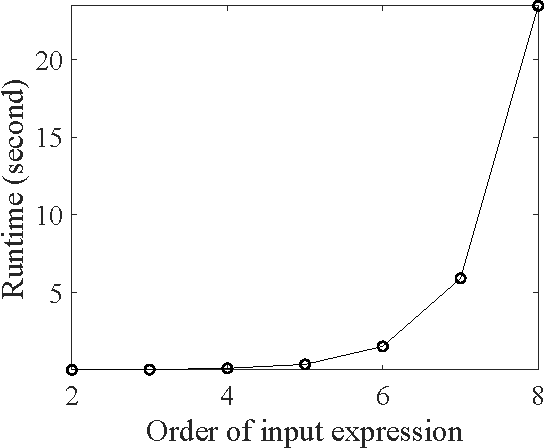
\includegraphics[width=0.45\textwidth]{fig/int-1.pdf}
    \label{order}
}
\subfigure[关于次数的运行时间]{
    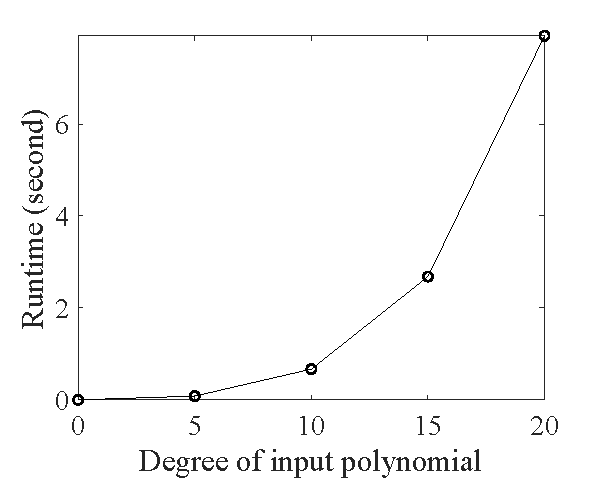
\includegraphics[width=0.45\textwidth]{fig/int-2.pdf}
    \label{degree}
}
\caption{IntSimplify 关于阶数和次数的运行时间}
\end{figure}

这似乎显得本文算法的时间复杂度过高. 但是, 在实际应用中很少有阶数超过8的积分表达式. 事实上, 考虑
\begin{equation}
\left(\int\!{(f_1\cdots f_n)_x\dd x}\right)^m,
\label{poly}
\end{equation}
其中 $f_1,\cdots,f_n$ 是互不相同的抽象函数. 上式的括号内部展开后有$M=2^n-1$项. 而将括号展开后将会产生$\binom{m+M-1}{m}$项, 其中 $\binom{A}{B}$是二项式系数. 从而, 对于这个例子, 本文算法的时间复杂度是 
\begin{equation}
\mathcal O\left(\binom{m+2^n-2}{m}^2\right).
\label{polynomial_complexity}    
\end{equation}
对于较大的$n$, 复杂度依然是指数的. 但是, 对于较小的$n$, 该复杂度等价于
$\mathcal O(m^{2N})$, 其中$N=2^n-2$. 换句话说, 在较小的阶数条件下, 本文算法的复杂度关于输入表达式的次数是多项式的. 这样的复杂度在实践中是能够被接受的. 在\refeqn{poly}中取$n=2,m\le 20$, 其运行时间如\reffig{degree}所示. 可以看出, 对于次数超过20的多项式, 我们的算法也能在8秒内完成求解. 

对于阶数和次数都较低的输入表达式, 本文算法的时间复杂度将进一步降低. 对于这样的输入, 我们的算法还有两种加速手段: 
\begin{asparaenum}[(I)]
\item 第一个加速手段是对计算结果建立记忆表. 在一般情况下, 不同的积分项可能有共同的组成部分, 从而使得它们在合并时的\emph{根情况}是相同的. 例如, 在例\ref{eg-4-1}中, $ad+bd=cd$ 和 $ac+bc=c^2$ 的\emph{根情况}都是 $a+b=c$. 如果我们对\emph{根情况}的计算结果建立记忆表, 当检测到重复运算时直接查表返回结果, 则能对计算进行加速. 这样的操作在Maple 中能够通过对函数加\cd{option remember}来简单地实现.
\item 第二个加速手段是对输入项进行分组后再合并. 我们注意到两个SII只有在有一样的$FR$时才能合并, 其中\begin{equation}    
FR(f)=\left\{
\begin{array}{cl}
\prod\limits_{g\in FC(f)}{FR(g)}, &\text{if }TP(f)=complex,\\ 
f,           &\text{if }TP(f)=simple.
\end{array}
\right.
\end{equation} 
所以, 可以按照$FR$将输入进行分组后再合并. 这能缩小搜索合并规则的范围, 从而加速计算. 
\end{asparaenum}

从\refeqn{polynomial_complexity}中可以看出, 当输入表达式的阶数和次数都有限时, 每个分组的化简时间是一个常数. 从而, 算法的时间复杂度关于输入规模是线性的. 

令 $\mathcal F=\{f_1,f_2,\cdots,f_n\}$, 考虑
\begin{equation}
\left(\sum\limits_{k=1}^{n_1}{\int\!{(f_{i_{2k-1}}f_{i_{2k}})_x\dd x}}\right)^4+\left(\sum\limits_{k=1}^{n_2}{\int\!{(f_{j_{3k-2}}f_{j_{3k-1}}f_{j_{3k}})_x\dd x}}\right)^2,
\label{construct}
\end{equation}
其中 $i_k,j_k \in \{1,2,\cdots,n\}$. 上式的次数是4, 且其阶数不超过$n$. 为了限制输入表达式的规模, 我们取$n=8,n_1\le 5,n_2\le 5$, 然后利用\cd{MatlabILP}进行优化, 运行时间如\reffig{items_all}所示.  

\begin{figure}[htbp]
\centering
\subfigure[不同输入项下的运行时间]{
    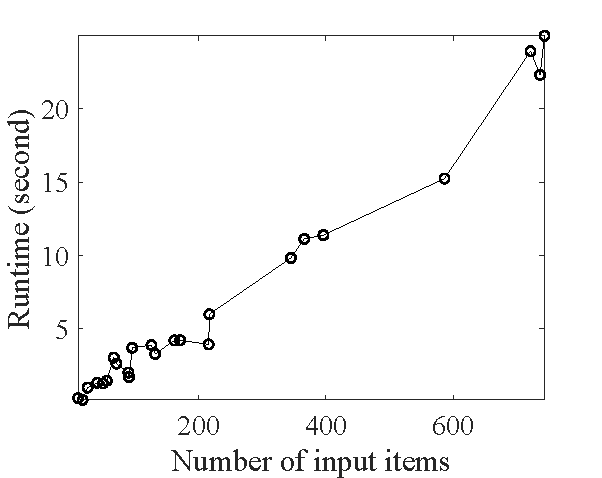
\includegraphics[width=0.45\textwidth]{fig/int-3.pdf}
    \label{items_input}
}
\subfigure[不同生成项下的运行时间]{
    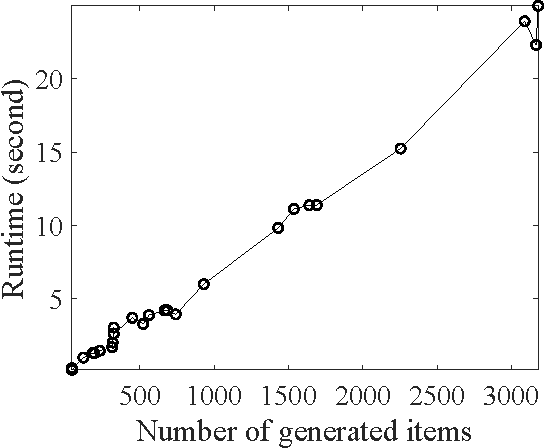
\includegraphics[width=0.45\textwidth]{fig/int-4.pdf}
    \label{items_gen}
}
\caption{IntSimplify 关于输入规模的运行时间}
\label{items_all}
\end{figure}

从\reffig{items_input}中可以看出, 运行时间关于输入项的增长是近似线性的. 从\reffig{items_gen}可以看出, 运行时间关于生成项的增长更加近似于线性. 运行时间有时随着项数的增长会发生下跌, 这是由记忆表策略造成的. 

综上所述, 在最差情况下, 我们的算法关于阶数的时间复杂度是指数的. 在有限的阶数条件下, \red{该算法复杂度的关于输入表达式的次数是多项式的}. 在阶数和次数都有限的情况下, 该算法的复杂度关于输入规模是线性的. 因此, 我们的算法在实际应用过程中往往是高效的.  

\section{小结} \label{Conclusion-03} 
因为在非线性微分方程求解的过程中往往需要进行非线性积分表达式的化简, 本文将非线性积分化简作为一个具有挑战性的任务进行研究. 本文基于导数的乘法规则提出了一个递归算法来寻找所有的二项合并规则, 基于这些规则, 将积分表达式化简的问题转化为一个精确线性规划问题进行求解. 最终, 本文实现的 IntSimplify 软件包能够化简线性不可约且含冗余项和嵌套积分的积分多项式, 解决了许多现有算法不能解决的问题.  

在对 IntSimplify 进行开发和测试的过程中, 我们还发现:
\begin{compactenum}[(1)]
\item 本文的算法关于输入表达式的阶数的时间复杂度是指数的, 关于次数的复杂度是多项式的, 关于输入规模的复杂度是线性的. 因此, 在阶数和次数都有限的情况下, 本文的算法往往是高效的.
\item 在求解对应的精确线性规划问题时, 由于数值计算带来的性能优势, 优秀的数值整数规划算法往往比一般的精确线性规划算法要快. 
\end{compactenum}

本章的研究成果已向  Proceedings of the 2019 ACM on International Symposium on Symbolic and Algebraic Computation 投稿, 目前正在审稿中.
